% =======================
% Agent Evaluation Section
% =======================
\section{Agent Evaluation}

% ---------------- Slide: From LLMs to Agents ----------------
\begin{frame}{From LLMs to Agents}

\begin{columns}[T]
\begin{column}{0.48\textwidth}
\textbf{LLM Application:}
\begin{itemize}
  \item Single model invocation
  \item Direct input $\rightarrow$ output
  \item Stateless (typically)
  \item Limited to text generation
\end{itemize}
\end{column}
\begin{column}{0.48\textwidth}
\textbf{Agent:}
\begin{itemize}
  \item Orchestrated system
  \item Multiple LLM calls
  \item Uses tools \& external systems
  \item Multi-step reasoning
  \item Maintains state across turns
\end{itemize}
\end{column}
\end{columns}

\vspace{0.5em}
\begin{center}
\small
\texttt{User} $\rightarrow$ \fbox{LLM$_1$} $\rightarrow$ \fbox{Tool} $\rightarrow$ \fbox{LLM$_2$} $\rightarrow$ \fbox{Action} $\rightarrow$ \texttt{Output}
\end{center}

\begin{block}{Evaluation Implication}
Increased complexity = more failure modes = more evaluation dimensions required.
\end{block}
\end{frame}

% ---------------- Slide: What is an Agent ----------------
\begin{frame}{Anatomy of an LLM Agent}

\begin{block}{Definition}
An \textbf{agent} is a system that uses an LLM as its reasoning engine to:
\begin{enumerate}
  \item Interpret user intent
  \item Plan a sequence of actions
  \item Execute actions using tools
  \item Observe results and iterate
\end{enumerate}
\end{block}

\textbf{Core Components:}
\begin{itemize}
  \item \textbf{Planner/Orchestrator}: Decides what to do next (LLM-based)
  \item \textbf{Tools}: External capabilities (APIs, databases, code execution)
  \item \textbf{Memory}: Context persistence across interactions
  \item \textbf{Guardrails}: Safety and policy constraints
\end{itemize}

\begin{block}{Agent Loop (Simplified)}
\texttt{Observe} $\rightarrow$ \texttt{Think} $\rightarrow$ \texttt{Act} $\rightarrow$ \texttt{Observe} $\rightarrow$ ...
\end{block}
\end{frame}

% ---------------- Slide: Examples of Agents ----------------
\begin{frame}{Examples of Agentic Applications}

\small
\begin{tabular}{p{2.8cm}p{4.2cm}p{3.5cm}}
\toprule
\textbf{Agent Type} & \textbf{Description} & \textbf{Key Evaluation Focus} \\
\midrule
Data Analysis Agent & Query databases, generate reports, create visualizations & Query correctness, data grounding \\
\addlinespace
Explainability Agent & Analyze code/models, explain inputs/outputs & Reasoning accuracy \\
\addlinespace
Document Intelligence & Extract, summarize, answer questions from documents & Extraction completeness, citation accuracy \\
\addlinespace
Coding Agent & Generate, review, debug, and execute code & Functional correctness, security \\
\addlinespace
Orchestrator Agent & Coordinate multiple sub-agents & Action sequencing, delegation accuracy \\
\addlinespace
Research Agent & Search, synthesize, and summarize information & Source quality, hallucination rate \\
\bottomrule
\end{tabular}

\end{frame}

% ---------------- Slide: What We Control ----------------
\begin{frame}{What We Control in Agent Systems}

\begin{tabular}{p{3.2cm}p{4cm}p{3cm}}
\toprule
\textbf{Control Point} & \textbf{Description} & \textbf{Optimization Goal} \\
\midrule
Agent Architecture & Number of agents, interaction patterns (sequential, parallel, hierarchical) & Right-size complexity \\
\addlinespace
Model per Agent & Which LLM for each sub-task & Cost/performance balance \\
\addlinespace
Agent Prompts & System instructions per agent & Task accuracy \\
\addlinespace
Tools / MCP & Available actions, APIs, data sources & Capability coverage \\
\addlinespace
Orchestration Logic & When to call which agent/tool & Efficiency, correctness \\
\bottomrule
\end{tabular}

\vspace{0.5em}
\begin{block}{Design Principle}
Find the \textbf{simplest and cheapest} combination of agents that solves your problem. More agents $\neq$ better.
\end{block}
\end{frame}

% ---------------- Slide: Why Agent Eval is Hard ----------------
\begin{frame}{Why Agent Evaluation is Challenging}

\textbf{Agents introduce new failure modes beyond single LLM calls:}

\begin{enumerate}
  \item \textbf{Multi-step dependencies}: Error in step 1 cascades to step N
  
  \item \textbf{Tool selection}: Agent may choose wrong tool or wrong parameters
  
  \item \textbf{State management}: Context may be lost or corrupted across turns
  
  \item \textbf{Non-determinism}: Same query can take different paths
  
  \item \textbf{Partial success}: Agent may complete 4/5 steps correctly
  
  \item \textbf{Side effects}: Actions may change external state (databases, APIs)
\end{enumerate}

\begin{block}{Key Insight}
A single accuracy metric is insufficient. We need \textbf{multi-dimensional evaluation} covering the full agent lifecycle.
\end{block}
\end{frame}

% ---------------- Slide: Metrics Taxonomy Overview ----------------
\begin{frame}{AI Metrics Taxonomy for Agents}

% Diagram placeholder - tikzpicture left empty intentionally
% \begin{center}
% \begin{tikzpicture}[
%   node distance=0.8cm,
%   box/.style={draw, rounded corners, minimum width=2cm, minimum height=0.6cm, font=\small}
% ]
% % Diagram content would go here
% \end{tikzpicture}
% \end{center}

\textbf{Hierarchical Relationship:}
$$
\text{Adoption} \xleftarrow{\text{depends on}} \text{Coverage} \xleftarrow{\text{within scope}} \begin{cases} \text{Accuracy} \\ \text{Latency} \\ \text{Cost} \end{cases}
$$

\begin{block}{Interpretation}
\begin{itemize}
  \item \textbf{Adoption} is the \textit{outcome} metric (downstream of quality)
  \item \textbf{Coverage} defines what the agent \textit{can} answer
  \item Within coverage, optimize for \textbf{Accuracy}, \textbf{Latency}, and \textbf{Cost}
\end{itemize}
\end{block}

\begin{block}{Warning}
Never interpret adoption in isolation---declining adoption signals coverage or quality issues.
\end{block}
\end{frame}

% ---------------- Slide: Metrics Definitions ----------------
\begin{frame}{Agent Metrics: Definitions}

\small
\begin{tabular}{p{2cm}p{5cm}p{3.2cm}}
\toprule
\textbf{Metric} & \textbf{Definition} & \textbf{How Measured} \\
\midrule
\textbf{Adoption} & User engagement with the agent & Unique users, queries/user, return rate, session length \\
\addlinespace
\textbf{Coverage} & Percentage of in-scope queries the agent can handle & \% handled vs. refused or failed \\
\addlinespace
\textbf{Latency} & Time from query to complete response & Time to first token, total time, \# of turns \\
\addlinespace
\textbf{Accuracy} & Correctness, completeness, and safety of responses & Using the Accuracy Bridge taxonomy \\
\addlinespace
\textbf{Cost} & Resource consumption per query & \$/query, tokens used, API calls, compute \\
\bottomrule
\end{tabular}

\vspace{0.5em}
\begin{block}{Trade-offs}
Improving accuracy may increase latency and cost. Optimizing cost may reduce accuracy. Evaluation must consider all dimensions.
\end{block}
\end{frame}

% ---------------- Slide: Coverage Deep Dive ----------------
\begin{frame}{Coverage: Defining Agent Scope}

\textbf{Coverage} = the spectrum of queries the agent is designed to handle.

\begin{block}{Expected Behaviors}
\begin{itemize}
  \item \textbf{In-scope query}: Agent should provide accurate, complete response
  \item \textbf{Out-of-scope query}: Agent should \textit{explicitly refuse}
  \begin{itemize}
    \item ``I'm not able to answer this question.''
    \item ``This is outside my capabilities. Please contact [X].''
  \end{itemize}
\end{itemize}
\end{block}

\textbf{Coverage Analysis:}
\begin{enumerate}
  \item Log all user queries (in-scope and out-of-scope)
  \item Analyze out-of-scope queries to distinguish:
  \begin{itemize}
    \item True misuse (user asking wrong agent)
    \item Capability gap (should be in scope, but isn't)
  \end{itemize}
  \item Use gaps to inform roadmap and expand evaluation dataset
\end{enumerate}

\begin{block}{Key Insight}
Graceful refusal is \textbf{correct behavior}---test for it explicitly.
\end{block}
\end{frame}

% ---------------- Slide: Latency Deep Dive ----------------
\begin{frame}{Latency: Breaking Down Response Time}

\textbf{Latency} can be decomposed into multiple components:

\begin{center}
\small
\begin{tabular}{p{3.5cm}p{6.5cm}}
\toprule
\textbf{Component} & \textbf{Definition} \\
\midrule
Time to First Token (TTFT) & Time until agent starts responding \\
Total Response Time & Time from query to complete response \\
Per-Tool Latency & Time spent in each tool invocation \\
Number of Turns & Conversation rounds to reach answer \\
Planning Time & Time spent in reasoning/orchestration \\
\bottomrule
\end{tabular}
\end{center}

\begin{block}{Context-Dependent Thresholds}
Acceptable latency depends on use case:
\begin{itemize}
  \item Interactive chat: $<5$ seconds expected
  \item Complex analysis: Minutes may be acceptable
  \item Background task: Hours may be fine
\end{itemize}
\end{block}

Define latency thresholds \textbf{per task type} in your evaluation criteria.
\end{frame}

% ---------------- Slide: Accuracy Bridge Intro ----------------
\begin{frame}{Accuracy: Beyond a Single Number}

\textbf{Challenge:} ``The agent was 85\% accurate'' doesn't enable improvement.

\begin{block}{The Accuracy Bridge}
A standardized taxonomy that decomposes inaccuracies into:
\begin{enumerate}
  \item \textbf{Failure Type}: What went wrong (user-visible outcome)
  \item \textbf{Root Cause}: Why it went wrong (technical origin)
  \item \textbf{Example}: Concrete illustration
\end{enumerate}
\end{block}

\textbf{Benefits:}
\begin{itemize}
  \item \textbf{Actionable}: Links failure type to fix (prompting? tools? retrieval?)
  \item \textbf{Comparable}: Same taxonomy across different agents
  \item \textbf{Trackable}: Monitor if fixes reduce specific failure types over time
  \item \textbf{Reportable}: Aggregated view for stakeholders
\end{itemize}
\end{frame}

% ---------------- Slide: Accuracy Bridge Table 1 ----------------
\begin{frame}{The Accuracy Bridge: Failure Taxonomy (1/2)}

\scriptsize
\begin{tabular}{p{1.8cm}p{3cm}p{2.8cm}p{2.8cm}}
\toprule
\textbf{Failure Type} & \textbf{Description} & \textbf{Root Causes} & \textbf{Example} \\
\midrule
\textbf{Hallucination} (Factually Wrong) & Information that is incorrect or not grounded in source data & Prompting, Retrieval, Tool error, Model limitation, Data quality & Agent returns incorrect value for a metric \\
\addlinespace
\textbf{Incomplete} & Response omits critical information required to answer & Prompting, Orchestration, Retrieval, Model limitation & Agent explains variance but omits primary driver \\
\addlinespace
\textbf{Extra Information} & Includes unrequested, irrelevant information & Prompting, Model limitation & Agent adds unrelated suggestions to a factual query \\
\addlinespace
\textbf{Wrong Format} & Content correct, but format doesn't match request & Prompting, Output schema, Model limitation & Returns paragraph when table was requested \\
\bottomrule
\end{tabular}
\end{frame}

% ---------------- Slide: Accuracy Bridge Table 2 ----------------
\begin{frame}{The Accuracy Bridge: Failure Taxonomy (2/2)}

\scriptsize
\begin{tabular}{p{1.8cm}p{3cm}p{2.8cm}p{2.8cm}}
\toprule
\textbf{Failure Type} & \textbf{Description} & \textbf{Root Causes} & \textbf{Example} \\
\midrule
\textbf{Wrong Action} & Executes incorrect, unintended, or unsafe state-changing action & Orchestration logic, Prompting, Tool config, Missing guardrails & Agent updates wrong record in database \\
\addlinespace
\textbf{Throttling / Timeout} & Fails to complete due to rate or time limits & Infrastructure limits, Retry logic, Token constraints, Tool latency & Agent stops mid-reasoning, returns error \\
\addlinespace
\textbf{Unsafe / Policy Violation} & Response or action violates safety, compliance, or policy & Prompting, Missing guardrails, Tool misuse, Model limitation & Agent exposes restricted data or performs unauthorized action \\
\bottomrule
\end{tabular}

\vspace{0.5em}
\begin{block}{Using the Accuracy Bridge}
When labeling an inaccurate response:
\begin{enumerate}
  \item Assign exactly one \textbf{failure type}
  \item Identify the most likely \textbf{root cause}
  \item This enables targeted fixes and trend analysis
\end{enumerate}
\end{block}
\end{frame}

% ---------------- Slide: Root Cause Mapping ----------------
\begin{frame}{Root Cause $\rightarrow$ Remediation Mapping}

\begin{center}
\small
\begin{tabular}{p{3cm}p{7cm}}
\toprule
\textbf{Root Cause} & \textbf{Typical Remediation} \\
\midrule
\textbf{Prompting} & Refine system prompt, add examples, improve instructions \\
\addlinespace
\textbf{Retrieval (RAG)} & Improve chunking, embedding model, retrieval strategy \\
\addlinespace
\textbf{Tool Configuration} & Fix tool parameters, add validation, improve tool descriptions \\
\addlinespace
\textbf{Orchestration Logic} & Adjust agent routing, improve planning prompts \\
\addlinespace
\textbf{Missing Guardrails} & Add input/output validation, safety filters \\
\addlinespace
\textbf{Model Limitation} & Try different model, add reasoning steps, decompose task \\
\addlinespace
\textbf{Data Quality} & Fix upstream data, add data validation \\
\addlinespace
\textbf{Infrastructure} & Increase limits, add retries, optimize for latency \\
\bottomrule
\end{tabular}
\end{center}

\begin{block}{Feedback Loop}
Accuracy Bridge $\rightarrow$ Root Cause Analysis $\rightarrow$ Targeted Fix $\rightarrow$ Re-evaluate
\end{block}
\end{frame}

% ---------------- Slide: Offline vs Online ----------------
\begin{frame}{Two Evaluation Modes: Offline and Online}

\begin{columns}[T]
\begin{column}{0.48\textwidth}
\textbf{Offline Evaluation}\\
(Pre-Deployment)
\begin{itemize}
  \item Run agent against curated dataset
  \item Ground truth available
  \item Controlled environment
  \item Gate for deployment
  \item Catch issues \textit{before} users see them
\end{itemize}
\end{column}
\begin{column}{0.48\textwidth}
\textbf{Online Evaluation}\\
(Post-Deployment)
\begin{itemize}
  \item Monitor production traffic
  \item Ground truth often unavailable
  \item Real user behavior
  \item Continuous monitoring
  \item Catch issues \textit{in the wild}
\end{itemize}
\end{column}
\end{columns}

\vspace{0.5em}
\begin{block}{Both Are Required}
\begin{itemize}
  \item Offline: Necessary but not sufficient (can't anticipate all real queries)
  \item Online: Catches drift, edge cases, and unexpected user behavior
\end{itemize}
\end{block}
\end{frame}

% ---------------- Slide: Offline Workflow ----------------
\begin{frame}{Offline Evaluation Workflow}

\textbf{Step-by-Step Process:}

\begin{enumerate}
  \item \textbf{Create Evaluation Dataset}
  \begin{itemize}
    \item Representative of expected production queries
    \item Include edge cases and adversarial examples
    \item Include out-of-scope queries (refusal = correct)
    \item Ground truth labels from domain experts (SMEs)
  \end{itemize}
  
  \item \textbf{Run Agent Against Dataset}
  \begin{itemize}
    \item Execute full agent pipeline (tools, reasoning, output)
    \item Capture all traces: prompts, tool calls, intermediate steps
  \end{itemize}
  
  \item \textbf{Evaluate and Label}
  \begin{itemize}
    \item Compute metrics (coverage, accuracy, latency, cost)
    \item Label failures using Accuracy Bridge
  \end{itemize}
  
  \item \textbf{Decision Gate}
  \begin{itemize}
    \item Meets quality bar? $\rightarrow$ Deploy
    \item Below bar? $\rightarrow$ Iterate (prompts, tools, architecture)
  \end{itemize}
\end{enumerate}
\end{frame}

% ---------------- Slide: Building Eval Dataset ----------------
\begin{frame}{Building a High-Quality Evaluation Dataset}

\textbf{Best Practices:}

\begin{columns}[T]
\begin{column}{0.48\textwidth}
\textbf{Do:}
\begin{itemize}
  \item[\checkmark] Define expected output for each input
  \item[\checkmark] Include diverse query types
  \item[\checkmark] Add edge cases and ambiguous inputs
  \item[\checkmark] Include multi-turn conversations
  \item[\checkmark] Test refusal behavior (out-of-scope)
  \item[\checkmark] Use SMEs for ground truth
  \item[\checkmark] Consider cost of mistakes per category
\end{itemize}
\end{column}
\begin{column}{0.48\textwidth}
\textbf{Don't:}
\begin{itemize}
  \item[$\times$] Only happy-path scenarios
  \item[$\times$] Homogeneous query types
  \item[$\times$] Ground truth without SME review
  \item[$\times$] Static dataset (never updated)
  \item[$\times$] Ignore tool invocation correctness
\end{itemize}
\end{column}
\end{columns}

\vspace{0.5em}
\begin{block}{Synthetic Data Generation}
Use an LLM to generate diverse test queries based on your agent's scope. Human review is still required for ground truth labels.
\end{block}
\end{frame}

% ---------------- Slide: Version Control ----------------
\begin{frame}{Versioning: Experiments and Datasets}

\textbf{Critical Practice:} Version \textit{both} the agent and the evaluation dataset.

\begin{block}{What to Version}
\begin{itemize}
  \item \textbf{Agent Configuration}
  \begin{itemize}
    \item Model(s) used, prompts, tool configurations
    \item Orchestration logic, parameters
  \end{itemize}
  \item \textbf{Evaluation Dataset}
  \begin{itemize}
    \item Input queries, expected outputs, labels
    \item Dataset version ID, creation date, author
  \end{itemize}
  \item \textbf{Results}
  \begin{itemize}
    \item Metrics per experiment run
    \item Mapping: Agent version $\times$ Dataset version $\rightarrow$ Metrics
  \end{itemize}
\end{itemize}
\end{block}

\begin{block}{Why It Matters}
Enables: reproducibility, regression detection, A/B comparison, audit trails.
\end{block}
\end{frame}

% ---------------- Slide: Online Workflow ----------------
\begin{frame}{Online Evaluation Workflow}

\textbf{Post-Deployment Monitoring:}

\begin{enumerate}
  \item \textbf{Automatic Telemetry Capture}
  \begin{itemize}
    \item Log all interactions: queries, outputs, tool calls, reasoning
    \item Capture latency per step, total cost, tokens used
    \item Collect user feedback (thumbs up/down, explicit ratings)
  \end{itemize}
  
  \item \textbf{Trace Review} (choose based on volume)
  \begin{itemize}
    \item \textit{Low volume}: Review all traces manually
    \item \textit{Medium volume}: Use LLM-as-a-Judge to flag, then human review
    \item \textit{High volume}: Sample (stratified), then LLM-as-a-Judge + human review
  \end{itemize}
  
  \item \textbf{Label Using Accuracy Bridge}
  \begin{itemize}
    \item Enables root cause analysis
    \item Feeds directly into reporting
  \end{itemize}
  
  \item \textbf{Export to Offline Dataset}
  \begin{itemize}
    \item Labeled production traces become new test cases
  \end{itemize}
\end{enumerate}
\end{frame}

% ---------------- Slide: User Feedback ----------------
\begin{frame}{Leveraging User Feedback}

\textbf{Types of User Signals:}

\begin{tabular}{p{3cm}p{4cm}p{3cm}}
\toprule
\textbf{Signal} & \textbf{What It Captures} & \textbf{Limitation} \\
\midrule
Thumbs Up/Down & Binary satisfaction & No detail on \textit{why} \\
Star Rating & Graded satisfaction & Still lacks specifics \\
Free-text Feedback & Detailed user input & Unstructured, hard to aggregate \\
Explicit Corrections & What should have been said & High signal, rare \\
Implicit Signals & Retry, abandon, escalate & Requires inference \\
\bottomrule
\end{tabular}

\vspace{0.5em}
\begin{block}{Best Practice}
\begin{itemize}
  \item Use \textbf{thumbs-down} as a prioritization signal for manual review
  \item Don't rely solely on feedback---users don't always report errors
  \item Combine with automated flagging (LLM-as-a-Judge)
\end{itemize}
\end{block}
\end{frame}

% ---------------- Slide: LLM as a Judge Intro ----------------
\begin{frame}{LLM-as-a-Judge: Scaling Evaluation}

\textbf{Concept:} Use an LLM to evaluate another LLM or agent's outputs.

\begin{block}{Two Operating Modes}
\begin{center}
\begin{tabular}{p{2cm}p{4cm}p{4cm}}
\toprule
\textbf{Mode} & \textbf{Offline (with ground truth)} & \textbf{Online (no ground truth)} \\
\midrule
Input & Query + Agent Output + Expected Output & Query + Agent Output + Trace \\
Task & Score against reference & Flag likely issues \\
Use Case & Automate scoring at scale & Prioritize traces for review \\
\bottomrule
\end{tabular}
\end{center}
\end{block}

\begin{block}{Critical Requirement}
LLM-as-a-Judge must be \textbf{calibrated} against human-labeled data. Human labeling remains the source of truth.
\end{block}
\end{frame}

% ---------------- Slide: LLM as a Judge Design ----------------
\begin{frame}{Designing an LLM-as-a-Judge}

\textbf{Key Design Decisions:}

\begin{enumerate}
  \item \textbf{Judge Model Selection}
  \begin{itemize}
    \item Often use a stronger/different model than the agent
    \item Trade-off: cost vs. reliability
  \end{itemize}
  
  \item \textbf{Judge Prompt Engineering}
  \begin{itemize}
    \item Define evaluation criteria explicitly
    \item Provide rubric with examples
    \item Request structured output (scores + reasoning)
  \end{itemize}
  
  \item \textbf{Calibration Process}
  \begin{itemize}
    \item Run judge on human-labeled gold set
    \item Measure agreement rate (Cohen's Kappa, accuracy)
    \item Set threshold: only deploy if agreement $> X\%$
  \end{itemize}
  
  \item \textbf{Ongoing Monitoring}
  \begin{itemize}
    \item Periodically re-validate against new human labels
    \item Watch for judge drift
  \end{itemize}
\end{enumerate}
\end{frame}

% ---------------- Slide: LLM as a Judge Pitfalls ----------------
\begin{frame}{LLM-as-a-Judge: Pitfalls and Mitigations}

\begin{tabular}{p{3.5cm}p{6.5cm}}
\toprule
\textbf{Pitfall} & \textbf{Mitigation} \\
\midrule
\textbf{Self-preference bias} & Judge favors outputs similar to its own style. Use different model family for judge. \\
\addlinespace
\textbf{Position bias} & In pairwise comparison, judge prefers first/second option. Randomize order, average scores. \\
\addlinespace
\textbf{Verbosity bias} & Longer responses rated higher regardless of quality. Explicitly instruct to ignore length. \\
\addlinespace
\textbf{Lack of calibration} & Judge disagrees with humans. Mandatory calibration on gold set before deployment. \\
\addlinespace
\textbf{Domain blindness} & Judge lacks domain expertise. Include domain context in prompt, or use domain-specific judge. \\
\bottomrule
\end{tabular}

\begin{block}{Golden Rule}
Never fully automate evaluation with LLM-as-a-Judge without ongoing human validation.
\end{block}
\end{frame}

% ---------------- Slide: Judge Example 1 (No Ground Truth) ----------------
\begin{frame}[fragile]{LLM-as-a-Judge Example: Hallucination Detection (No Ground Truth)}

\scriptsize
\textbf{Use Case:} When ground truth is unavailable, judge evaluates plausibility and factual consistency.

\vspace{0.3em}
\begin{block}{Judge Prompt}
\tiny
\texttt{Evaluate the degree of hallucination in the generation on a continuous scale from 0 to 1.}

\texttt{A generation can be considered to hallucinate (Score: 1) if it does not align with established}
\texttt{knowledge, verifiable data, or logical inference, and often includes elements that are}
\texttt{implausible, misleading, or entirely fictional.}

\vspace{0.2em}
\textbf{Example:}
\begin{itemize}
  \item Query: \textit{Can eating carrots improve your vision?}
  \item Generation: \textit{Yes, eating carrots significantly improves your vision, especially at night...}
  \item Score: 1.0
  \item Reasoning: \textit{Carrots only improve vision under specific circumstances (vitamin A deficiency).}
\end{itemize}

\vspace{0.2em}
\textbf{Input Template:}
\texttt{Query: \{\{query\}\} | Generation: \{\{generation\}\} | Think step by step.}
\end{block}

\begin{block}{Key Insight}
Without ground truth, the judge relies on world knowledge and logical consistency.
\end{block}
\end{frame}

% ---------------- Slide: Judge Example 2 (With Ground Truth) ----------------
\begin{frame}[fragile]{LLM-as-a-Judge Example: Correctness Evaluation (With Ground Truth)}

\scriptsize
\textbf{Use Case:} When ground truth is available, judge compares generation against reference answer.

\vspace{0.3em}
\begin{block}{Judge Prompt}
\tiny
\texttt{Evaluate the correctness of the generation on a continuous scale from 0 to 1.}

\texttt{A generation can be considered correct (Score: 1) if it includes all the key facts from the}
\texttt{ground truth and if every fact presented is factually supported by the ground truth or common sense.}

\vspace{0.2em}
\textbf{Example:}
\begin{itemize}
  \item Query: \textit{Can eating carrots improve your vision?}
  \item Generation: \textit{Yes, eating carrots significantly improves your vision...} (same as before)
  \item Ground Truth: \textit{Carrots contain beta-carotene (vitamin A). Extreme lack causes blindness.}
  \item Score: 0.1
  \item Reasoning: \textit{Generation mentions vision improvement but fails to explain the mechanism or circumstances. Contains misinformation and exaggerations.}
\end{itemize}

\vspace{0.2em}
\textbf{Input Template:}
\texttt{Query: \{\{query\}\} | Generation: \{\{generation\}\} | Ground truth: \{\{ground\_truth\}\}}
\end{block}

\begin{block}{Key Insight}
With ground truth, scoring is more objective and can catch subtle omissions or additions.
\end{block}
\end{frame}

% ---------------- Slide: Langfuse HLD ----------------
\begin{frame}{Production Agent Evaluation: A Two-Phase System}

\scriptsize

\begin{center}
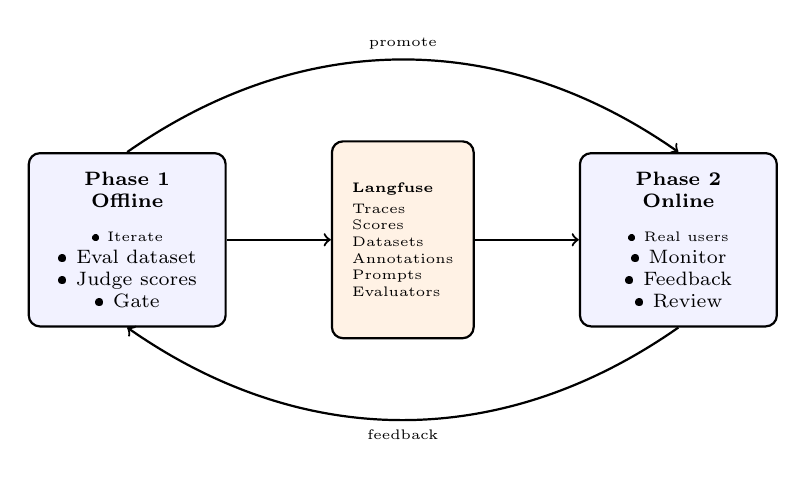
\begin{tikzpicture}[
  node distance=0.6cm,
  phase/.style={rectangle, draw, thick, rounded corners, minimum width=2.5cm, minimum height=2.2cm, font=\scriptsize, align=center, fill=blue!5},
  langfuse/.style={rectangle, draw, thick, rounded corners, minimum width=1.8cm, minimum height=2.5cm, font=\tiny, align=left, fill=orange!10},
  arrow/.style={->, thick}
]

% Phase 1: Offline (Beta)
\node[phase] (beta) at (0,0) {
  \textbf{Phase 1}\\
  \textbf{Offline}\\[0.15cm]
  \tiny
  • Iterate\\
  • Eval dataset\\
  • Judge scores\\
  • Gate
};

% Langfuse in the center
\node[langfuse] (langfuse) at (3.5,0) {
  \textbf{Langfuse}\\[0.05cm]
  \tiny
  Traces\\
  Scores\\
  Datasets\\
  Annotations\\
  Prompts\\
  Evaluators
};

% Phase 2: Online (Prod)
\node[phase] (prod) at (7,0) {
  \textbf{Phase 2}\\
  \textbf{Online}\\[0.15cm]
  \tiny
  • Real users\\
  • Monitor\\
  • Feedback\\
  • Review
};

% Arrows
\draw[arrow] (beta.east) -- (langfuse.west);
\draw[arrow] (langfuse.east) -- (prod.west);
\draw[arrow, bend left=35] (beta.north) to node[above, font=\tiny] {promote} (prod.north);
\draw[arrow, bend left=35] (prod.south) to node[below, font=\tiny] {feedback} (beta.south);

\end{tikzpicture}
\end{center}

\vspace{0.4em}
\begin{columns}[T]
\begin{column}{0.48\textwidth}
\textbf{Offline (Beta):}
\begin{itemize}
  \item Experiment on eval datasets
  \item LLM-as-a-Judge automated scoring
  \item Accuracy gate before promotion
\end{itemize}
\end{column}
\begin{column}{0.48\textwidth}
\textbf{Online (Production):}
\begin{itemize}
  \item Continuous trace monitoring
  \item User feedback collection
  \item Weekly human review
\end{itemize}
\end{column}
\end{columns}

\vspace{0.3em}
\begin{block}{Key Insight}
Production failures feed back into the evaluation dataset, creating continuous improvement.
\end{block}

\end{frame}

% ---------------- Slide: Sampling Strategies ----------------
\begin{frame}{Sampling Strategies for High-Volume Agents}

\textbf{Problem:} Can't manually review every trace when volume is high.

\begin{block}{Sampling Approaches}
\begin{enumerate}
  \item \textbf{Random Sampling}
  \begin{itemize}
    \item Simple, unbiased estimate of overall quality
    \item May miss rare but important failure modes
  \end{itemize}
  
  \item \textbf{Stratified Sampling}
  \begin{itemize}
    \item Sample proportionally across categories (query type, user segment)
    \item Ensures representation of all strata
  \end{itemize}
  
  \item \textbf{Importance Sampling}
  \begin{itemize}
    \item Oversample high-risk or high-value interactions
    \item Weight results to recover population estimates
  \end{itemize}
  
  \item \textbf{Signal-Based Sampling}
  \begin{itemize}
    \item Prioritize: thumbs-down, long latency, errors, LLM-as-a-Judge flags
  \end{itemize}
\end{enumerate}
\end{block}

Combine strategies: e.g., random baseline + signal-based enrichment.
\end{frame}

% ---------------- Slide: Closing the Loop ----------------
\begin{frame}{Closing the Feedback Loop}

\begin{center}
\textbf{Continuous Improvement Cycle}
\end{center}

$$
\boxed{\text{Offline Eval}} \xrightarrow{\text{pass}} \boxed{\text{Deploy}} \xrightarrow{\text{monitor}} \boxed{\text{Online Eval}}
$$
$$
\uparrow \hspace{6cm} \downarrow
$$
$$
\boxed{\text{Update Dataset}} \xleftarrow{\text{label \& export}} \boxed{\text{Review Traces}}
$$

\vspace{0.5em}
\textbf{Key Activities:}
\begin{enumerate}
  \item Label production failures using Accuracy Bridge
  \item Export labeled traces to offline evaluation dataset (new version)
  \item Test new agent versions against real failure modes
  \item Use for \textbf{non-regression testing}: ensure fixes don't break other cases
\end{enumerate}

\begin{block}{Result}
Over time, evaluation dataset reflects real production challenges $\rightarrow$ more robust pre-deployment testing.
\end{block}
\end{frame}

% ---------------- Slide: Feedback Loop Agent ----------------
\begin{frame}{Advanced: Automated Feedback Analysis}

\textbf{Concept:} Use an agent to analyze evaluation data and suggest improvements.

\begin{block}{Feedback Analysis Agent}
\textbf{Inputs:}
\begin{itemize}
  \item LLM-as-a-Judge scores
  \item Human labels (Accuracy Bridge categories)
  \item User feedback (thumbs up/down, comments)
  \item Agent traces and codebase structure
\end{itemize}

\textbf{Outputs:}
\begin{itemize}
  \item Pattern detection across failures (common root causes)
  \item Suggested prompt refinements
  \item Identified capability gaps
  \item Prioritized improvement opportunities
\end{itemize}
\end{block}

\textbf{Example Platforms:} Langfuse, LangSmith, Weights \& Biases Weave, custom solutions.
\end{frame}

% ---------------- Slide: Observability ----------------
\begin{frame}{Agent Observability: What to Capture}

\textbf{Comprehensive Tracing:}

\begin{tabular}{p{3cm}p{7cm}}
\toprule
\textbf{Component} & \textbf{What to Log} \\
\midrule
\textbf{Input} & User query, session ID, timestamp, user metadata \\
\textbf{Planning} & Reasoning steps, selected tools, agent routing decisions \\
\textbf{Tool Calls} & Tool name, parameters, response, latency, errors \\
\textbf{LLM Invocations} & Prompt, completion, model, tokens, latency, cost \\
\textbf{Output} & Final response, confidence signals, citations \\
\textbf{Feedback} & User rating, explicit feedback, implicit signals \\
\textbf{Metadata} & Agent version, experiment ID, environment \\
\bottomrule
\end{tabular}

\begin{block}{Design Principle}
Log at a granularity that enables \textbf{root cause analysis}. If you can't trace a failure to a specific step, you can't fix it.
\end{block}
\end{frame}

% ---------------- Slide: Reporting ----------------
\begin{frame}{Standardized Reporting}

\textbf{Example Status Report Structure:}

\begin{quote}
\small
``As of [date], Agent X can answer \textbf{X\%} of in-scope questions (Coverage). \textbf{X users} submitted \textbf{X queries} this period, $\pm$X\% vs.\ prior (Adoption). Average latency was \textbf{X seconds} over \textbf{X turns} (Latency). Total cost was \textbf{\$X} (Cost). Of \textbf{X reviewed interactions}, \textbf{Y} were inaccurate (Accuracy):
\begin{itemize}
  \item X cases: hallucination (root cause: retrieval)
  \item X cases: wrong action (root cause: tool config)
  \item X cases: timeout (root cause: infrastructure)
\end{itemize}
Corrective actions: ...''
\end{quote}

\begin{block}{Benefits of Standardization}
\begin{itemize}
  \item Comparable across agents
  \item Directly derived from Accuracy Bridge labels
  \item Enables trend tracking over time
\end{itemize}
\end{block}
\end{frame}

% ---------------- Slide: Common Risks ----------------
\begin{frame}{Common Risks in Agent Evaluation}

\begin{tabular}{p{2.5cm}p{4cm}p{4cm}}
\toprule
\textbf{Risk} & \textbf{Description} & \textbf{Mitigation} \\
\midrule
\textbf{Under-labeling} & Not enough traces reviewed & Set review targets, allocate dedicated time \\
\addlinespace
\textbf{Eval Set Gaming} & Eval dataset doesn't represent production & Follow best practices, continuously update from production \\
\addlinespace
\textbf{Judge Misuse} & LLM-as-a-Judge without calibration & Mandatory calibration, periodic re-validation \\
\addlinespace
\textbf{Metric Fixation} & Optimizing one metric at expense of others & Track all five dimensions, set balanced thresholds \\
\addlinespace
\textbf{Drift Blindness} & Not detecting degradation over time & Automated monitoring, scheduled audits \\
\bottomrule
\end{tabular}
\end{frame}

% ---------------- Slide: Tooling Landscape ----------------
\begin{frame}{Agent Evaluation Tooling Landscape}

\textbf{Open Source \& Commercial Platforms:}

\begin{tabular}{p{3cm}p{7cm}}
\toprule
\textbf{Tool} & \textbf{Key Capabilities} \\
\midrule
\textbf{Langfuse} & Tracing, scoring, prompt management, analytics \\
\textbf{LangSmith} & Tracing, evaluation, dataset management, hub \\
\textbf{Weights \& Biases} & Experiment tracking, Weave for LLM tracing \\
\textbf{Arize Phoenix} & Observability, evaluation, embedding analysis \\
\textbf{Braintrust} & Eval framework, scoring, CI/CD integration \\
\textbf{Ragas} & RAG-specific evaluation metrics \\
\textbf{DeepEval} & Unit testing framework for LLMs \\
\textbf{OpenAI Evals} & Evaluation framework and benchmarks \\
\bottomrule
\end{tabular}

\vspace{0.3em}
\begin{block}{Build vs. Buy}
Evaluate based on: integration needs, customization requirements, scale, and team expertise.
\end{block}
\end{frame}

% ---------------- Slide: Summary ----------------
\begin{frame}{Agent Evaluation: Key Takeaways}

\begin{enumerate}
  \item \textbf{Agents are complex systems} with more failure modes than single LLM calls
  
  \item \textbf{Multi-dimensional metrics}: Adoption, Coverage, Latency, Accuracy, Cost
  
  \item \textbf{Accuracy Bridge}: Standardized failure taxonomy enables actionable insights
  \begin{itemize}
    \item Failure Type $\rightarrow$ Root Cause $\rightarrow$ Targeted Fix
  \end{itemize}
  
  \item \textbf{Offline + Online}: Both required for comprehensive evaluation
  
  \item \textbf{LLM-as-a-Judge}: Scales evaluation but must be calibrated; humans remain source of truth
  
  \item \textbf{Close the loop}: Production failures $\rightarrow$ evaluation dataset $\rightarrow$ better agents
  
  \item \textbf{Observability is foundational}: Can't improve what you can't trace
  
  \item \textbf{Version everything}: Agent configs, datasets, and results
\end{enumerate}
\end{frame}

% ---------------- Slide: Comparison ----------------
\begin{frame}{LLM vs. Agent Evaluation: Summary Comparison}

\small
\begin{tabular}{p{3cm}p{4cm}p{4cm}}
\toprule
\textbf{Dimension} & \textbf{LLM Application} & \textbf{Agent} \\
\midrule
Complexity & Single model call & Multi-step, multi-component \\
Failure Modes & Output quality & + Tool selection, orchestration, state \\
Key Metrics & Task-specific (precision, recall, BLEU, etc.) & Adoption, Coverage, Latency, Accuracy, Cost \\
Accuracy Analysis & Binary or rubric-based & Accuracy Bridge taxonomy \\
Ground Truth & Often available offline & Harder to define for multi-step tasks \\
Observability & Input/output logging & Full trace: planning, tools, intermediate steps \\
Iteration Unit & Prompt version & Agent config (prompts + tools + orchestration) \\
\bottomrule
\end{tabular}

\vspace{0.5em}
\begin{block}{Unifying Principle}
Both require: systematic evaluation, continuous monitoring, feedback loops, and human oversight.
\end{block}
\end{frame}

% ---------------- Slide: Questions ----------------
\begin{frame}{Questions?}

\begin{block}{Key Resources}
\begin{itemize}
  \item Langfuse Documentation: \url{https://langfuse.com/docs}
  \item LangChain Evaluation Guide: \url{https://python.langchain.com/docs/guides/evaluation}
  \item ``Judging LLM-as-a-Judge'' (Zheng et al., 2023)
  \item RAGAS: \url{https://docs.ragas.io}
\end{itemize}
\end{block}

\vspace{1em}
\begin{center}
\Large
\textbf{Thank you!}
\end{center}
\end{frame}
